\usetikzlibrary{shapes,arrows}

\tikzstyle{input} = [coordinate]
\tikzstyle{output} = [coordinate]
\tikzstyle{block} = [draw, rectangle]
\tikzstyle{sum} = [draw, circle]

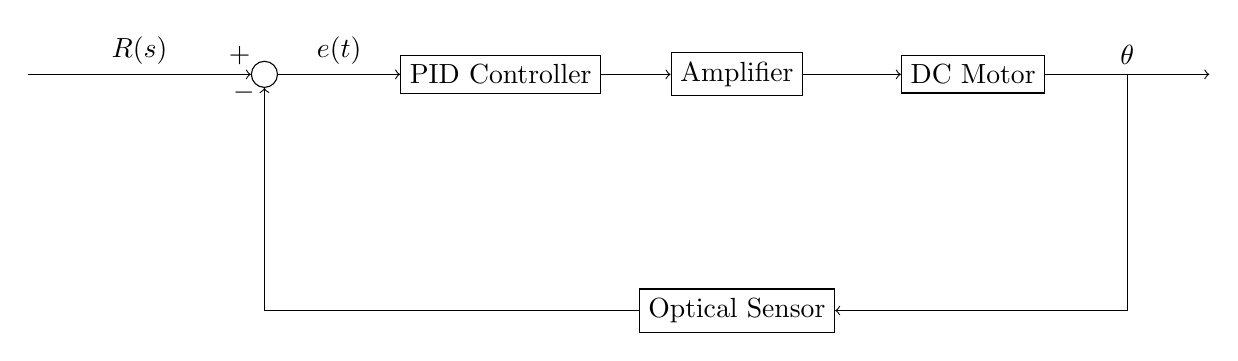
\begin{tikzpicture}[auto,node distance=3cm]
	% put the nodes (blocks, sums, etc..) where we want them
	\node [input,name=input] (in) {$\theta_d$};
	\node [sum,right of=in] (sum1) {};
	\node [block,right of=sum1] (g1) {PID Controller};
	\node [block,right of=g1] (g2) {Amplifier};
	\node [block,right of=g2] (g3) {DC Motor};
	\node [output,right of=g3] (out) {};
	\node [block,below of=g2] (h1) {Optical Sensor};

	% draw the feedforwards
	\draw [->] (in) -- node {$R(s)$} node[pos=0.95] {$+$} (sum1);
	\draw [->] (sum1) -- node {$e(t)$} (g1);
	\draw [->] (g1) -- (g2);
	\draw [->] (g2) -- (g3);
	\draw [->] (g3) -- node[name=p2] {$\theta$} (out);

	% h1 feedback
	\draw [->] (p2) |- (h1);
	\draw [->] (h1) -| node[pos=0.99] {$-$} (sum1);
	
\end{tikzpicture}

